%% Common definitions, defined in sdss-er.tex
\newlength{\pointonesec}\settowidth{\pointonesec}{$0.1$ s}
\newlength{\acceptable}\settowidth{\acceptable}{Acceptable}

\newcommand{\sdssertable}{\begin{tabular}{|c|D{.}{.}{6.0}|D{.}{.}{6.0}|D{.}{.}{3.2}|}
\hline
\multicolumn{1}{|c|}{\textbf{Phase}} & \multicolumn{1}{c|}{\textbf{Images recognized}} & \multicolumn{1}{c|}{\textbf{Unrecognized}} &
\multicolumn{1}{c|}{\textbf{Percent recognized}} \\
\hline
\usnob: \makebox[\pointonesec][r]{$0.1$ s} & 172,882 & 9,339 & 94.87 \\
\usnob: \makebox[\pointonesec][r]{$1$ s} & 181,826 & 395 & 99.78 \\
\usnob: \makebox[\pointonesec][r]{$10$ s} & 182,158 & 63 & 99.97 \\
\usnob: \makebox[\pointonesec][r]{$15$ s} & 182,160 & 61 & 99.97 \\
\twomass & 182,211 & 10 & 99.99 \\
Original images & 182,221 & 0 & 100.00 \\
\hline
\end{tabular}
}

\newcommand{\sdsserradecfig}{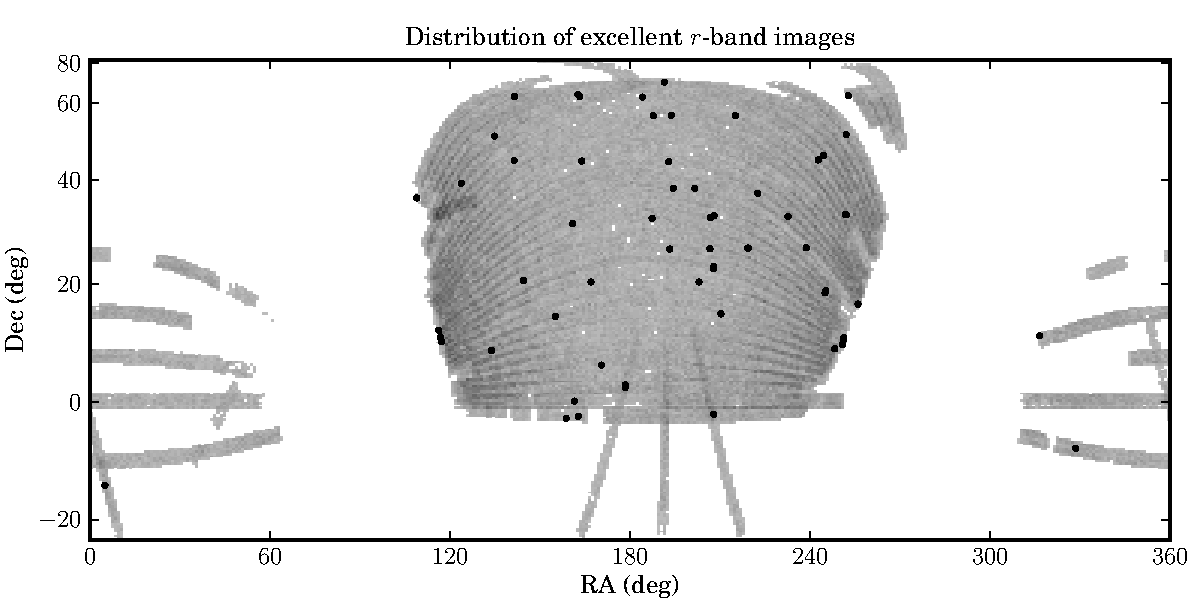
\includegraphics[width=2.000000\figunit]{sdss-er-radec}}
\newcommand{\sdssercputimefig}{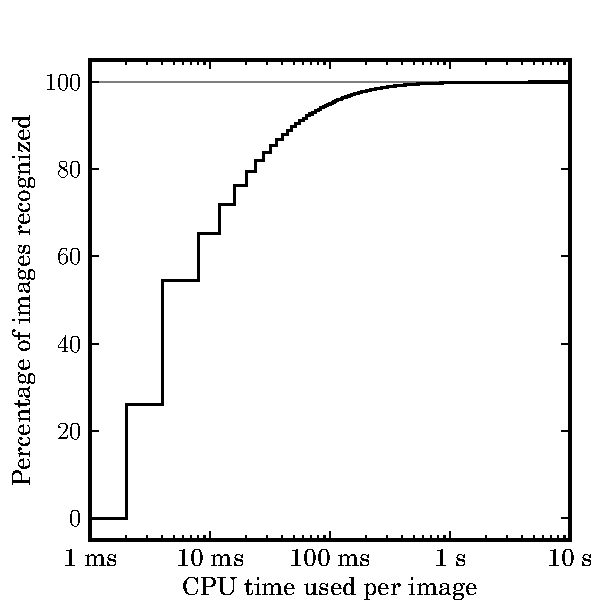
\includegraphics[width=1.000000\figunit]{sdss-er-cputime}}
\newcommand{\sdssernimagefig}{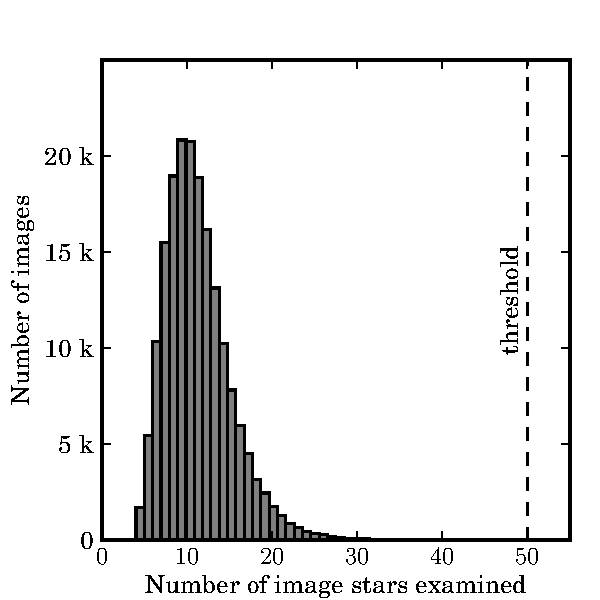
\includegraphics[width=1.000000\figunit]{sdss-er-nimage}}
\newcommand{\sdssernmatchfig}{\includegraphics[width=1.000000\figunit]{sdss-er-nmatch}}
\newcommand{\sdssercodeerrfig}{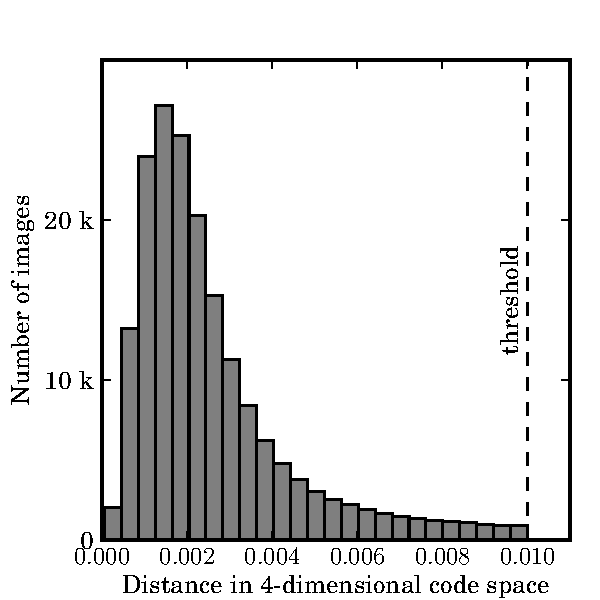
\includegraphics[width=1.000000\figunit]{sdss-er-codeerr}}
\newcommand{\sdsserbayesfig}{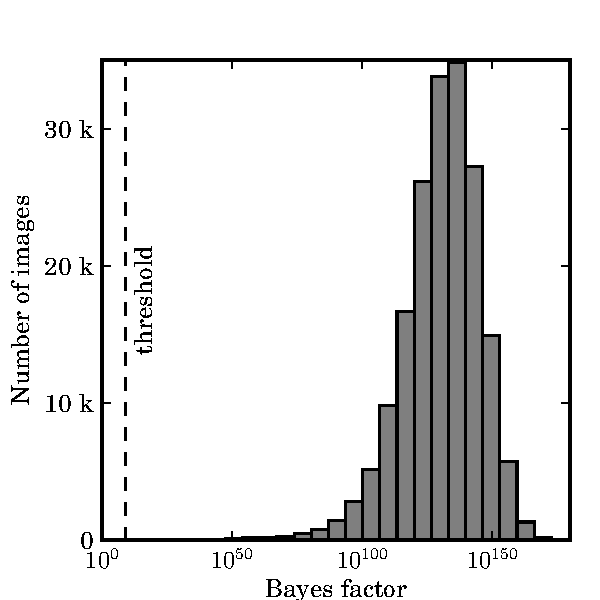
\includegraphics[width=1.000000\figunit]{sdss-er-bayes}}

\newcommand{\sdsserntoverifyfig}{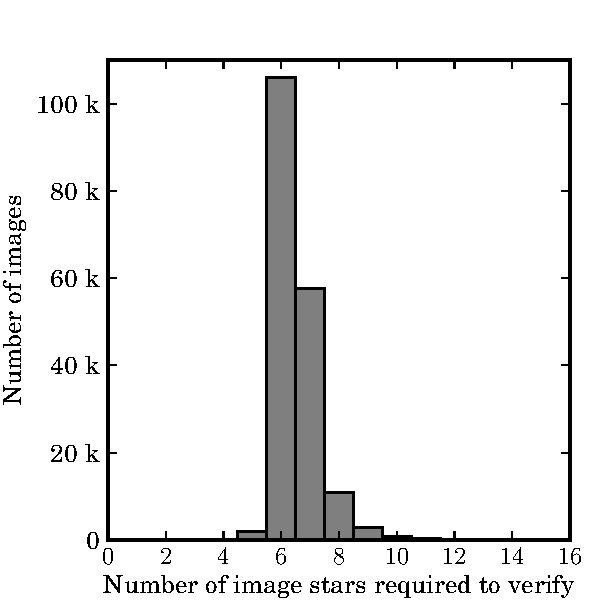
\includegraphics[width=1.000000\figunit]{sdss-er-ntoverify}}
\newcommand{\sdssbandtable}{\begin{tabular}{|c|D{.}{.}{3.2}|D{.}{.}{3.2}|D{.}{.}{3.2}|D{.}{.}{3.2}|D{.}{.}{3.2}|}
\hline
\multicolumn{1}{|c|}{\textbf{CPU time}} &\multicolumn{5}{c|}{\textbf{Percentage of images recognized}} \\
\cline{2-6}
\multicolumn{1}{|c|}{(per image)} & \multicolumn{1}{c|}{$u$} & \multicolumn{1}{c|}{$g$} & \multicolumn{1}{c|}{$r$} & \multicolumn{1}{c|}{$i$} & \multicolumn{1}{c|}{$z$} \\
\hline
\makebox[\pointonesec][r]{$0.1$ s} & 87.80  & 93.88  & 94.87  & 93.59  & 94.36 \\
\makebox[\pointonesec][r]{$1$ s} & 98.58  & 99.73  & 99.78  & 99.73  & 99.75 \\
\makebox[\pointonesec][r]{$10$ s} & 99.82  & 99.96  & 99.97  & 99.96  & 99.96 \\
\makebox[\pointonesec][r]{$60$ s} & 99.84  & 99.96  & 99.97  & 99.96  & 99.96 \\
\hline
\end{tabular}
}
\newcommand{\sdssbandsobjsfig}{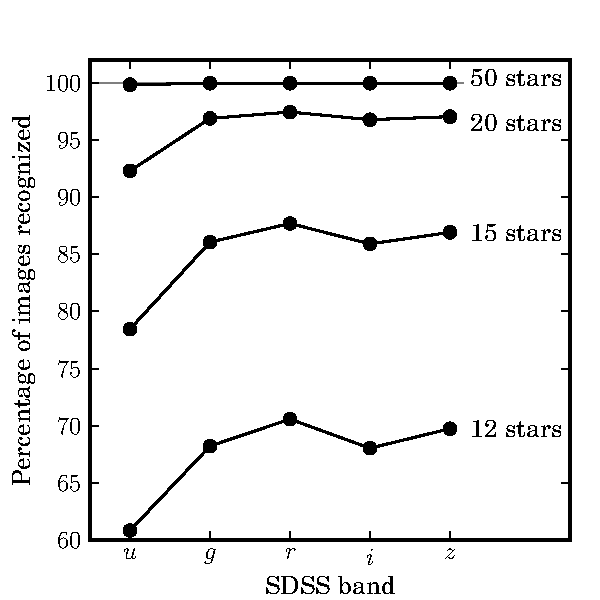
\includegraphics[width=1.000000\figunit]{sdss-bands-objs}}
\newcommand{\sdssbandstimefig}{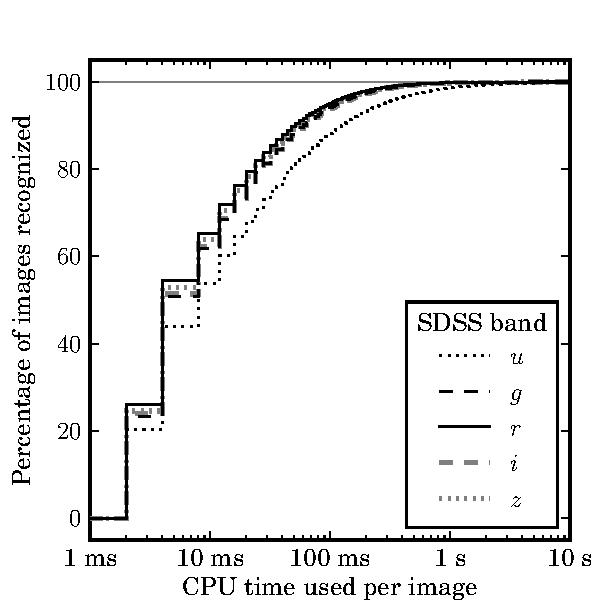
\includegraphics[width=1.000000\figunit]{sdss-bands-time}}
\newcommand{\sdssqualtable}{\begin{tabular}{|c|D{.}{.}{3.2}|D{.}{.}{3.2}|D{.}{.}{3.2}|D{.}{.}{3.2}|}
\hline
\multicolumn{1}{|c|}{\textbf{CPU time}} &\multicolumn{4}{c|}{\textbf{Percentage of images recognized}} \\
\cline{2-5}
\multicolumn{1}{|c|}{(per image)} & \multicolumn{1}{c|}{\makebox[\acceptable][c]{Excellent}} & \multicolumn{1}{c|}{\makebox[\acceptable][c]{Good}} & \multicolumn{1}{c|}{\makebox[\acceptable][c]{Acceptable}} & \multicolumn{1}{c|}{\makebox[\acceptable][c]{Bad}} \\
\hline
\makebox[\pointonesec][r]{$0.1$ s} & 94.87  & 94.85  & 94.57  & 84.11 \\
\makebox[\pointonesec][r]{$1$ s} & 99.78  & 99.74  & 99.64  & 96.58 \\
\makebox[\pointonesec][r]{$10$ s} & 99.97  & 99.94  & 99.94  & 99.11 \\
\makebox[\pointonesec][r]{$60$ s} & 99.97  & 99.94  & 99.95  & 99.18 \\
\hline
\end{tabular}
}
\newcommand{\sdssqualtimefig}{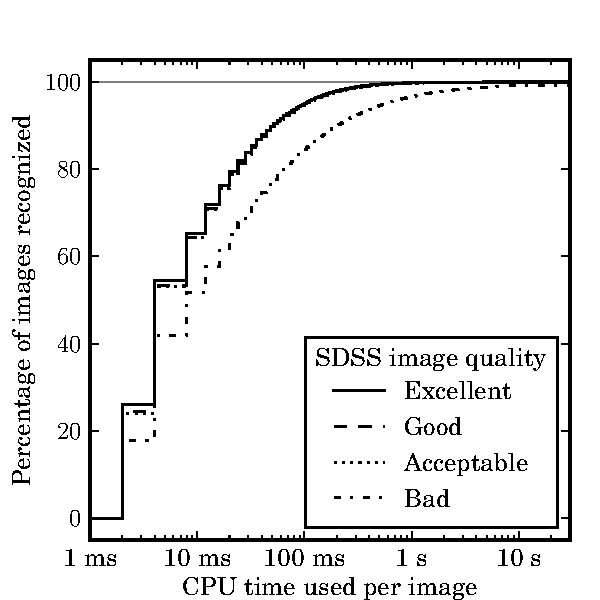
\includegraphics[width=1.000000\figunit]{sdss-qual-time}}
\newcommand{\sdssqualobjsfig}{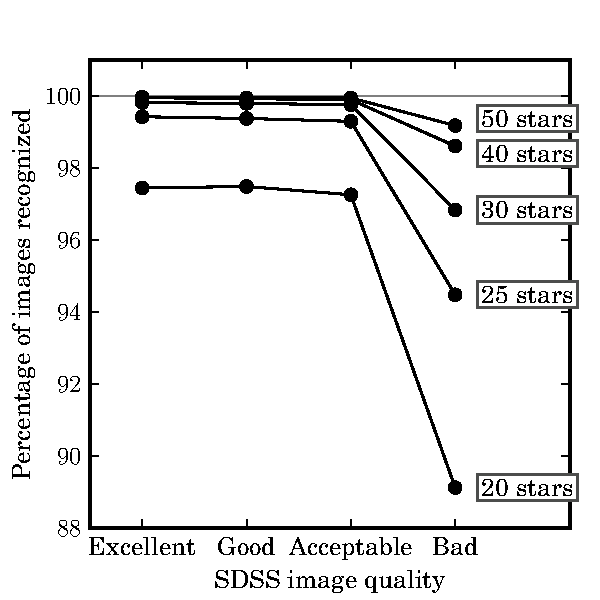
\includegraphics[width=1.000000\figunit]{sdss-qual-objs}}
\newcommand{\sdssimsizetimefig}{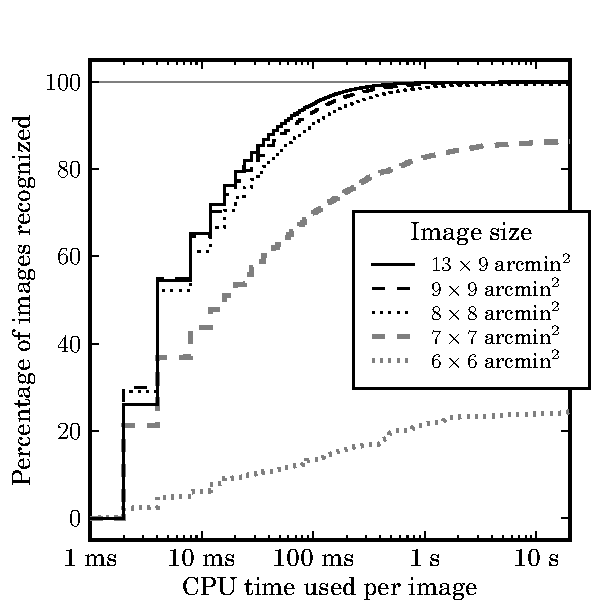
\includegraphics[width=1.000000\figunit]{sdss-imsize-time}}
\newcommand{\sdssimsizetable}{\begin{tabular}{|D{x}{\times}{2.1}|D{.}{.}{3.2}|}
\hline
\multicolumn{1}{|c|}{\textbf{Image size (arcmin${}^2$)}} &
\multicolumn{1}{c|}{\textbf{Percentage of images recognized}} \\
\hline
13x9 & 99.97\\
9x9 & 99.88\\
8x8 & 99.52\\
7x7 & 86.53\\
6x6 & 24.75\\
\hline
\end{tabular}
}
\newcommand{\sdssimsizeobjsfig}{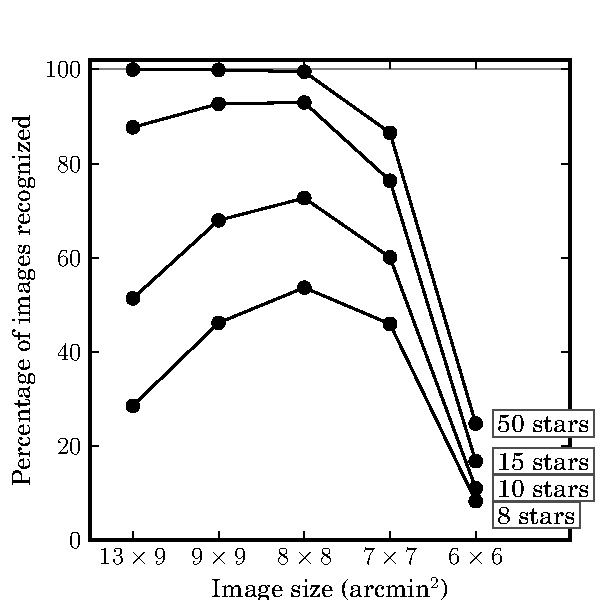
\includegraphics[width=1.000000\figunit]{sdss-imsize-objs}}
\newcommand{\sdsssizehintsreltimefig}{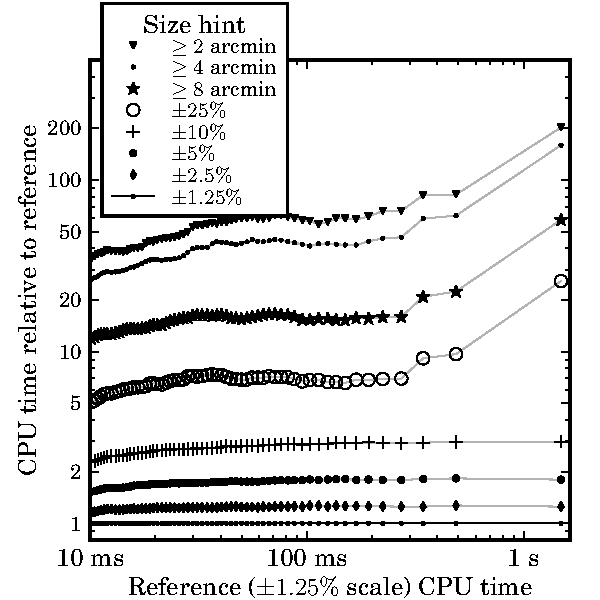
\includegraphics[width=1.000000\figunit]{sdss-sizehints-reltime}}
\newcommand{\sdsssizehintstimefig}{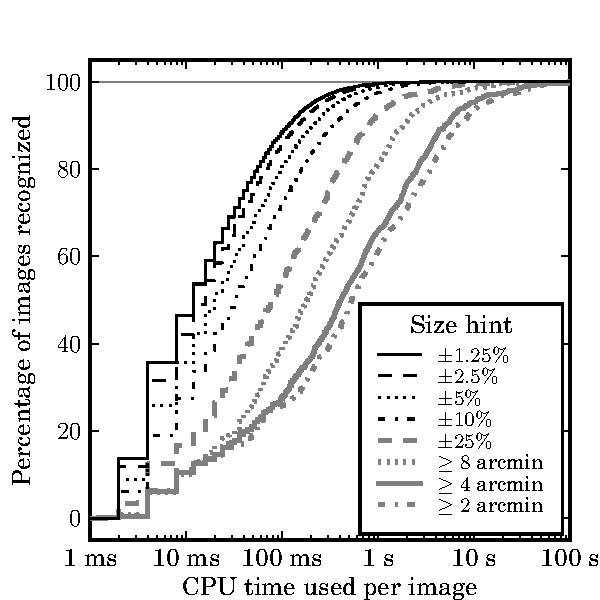
\includegraphics[width=1.000000\figunit]{sdss-sizehints-time}}
\newcommand{\sdsssizehintsindexfig}{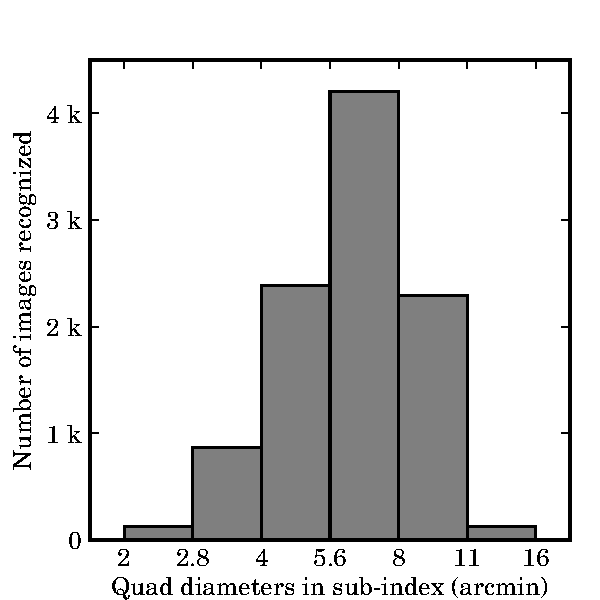
\includegraphics[width=1.000000\figunit]{sdss-sizehints-index}}
\newcommand{\sdssdensitytable}{\begin{tabular}{|c|D{.}{.}{3.2}|D{.}{.}{3.2}|D{.}{.}{3.2}|D{.}{.}{3.2}|D{.}{.}{3.2}|}
\hline
\multicolumn{1}{|c|}{\textbf{CPU time}} &\multicolumn{5}{c|}{\textbf{Percentage of images recognized}} \\
\cline{2-6}
\multicolumn{1}{|c|}{(per image)} & \multicolumn{1}{c|}{$16$ quads/cell} & \multicolumn{1}{c|}{$9$ quads/cell} & \multicolumn{1}{c|}{$4$ quads/cell} & \multicolumn{1}{c|}{$3$ quads/cell} & \multicolumn{1}{c|}{$2$ quads/cell} \\
\hline
\makebox[\pointonesec][r]{$0.1$ s} & 94.44  & 96.32  & 95.89  & 94.30  & 90.94 \\
\makebox[\pointonesec][r]{$1$ s} & 99.76  & 99.84  & 99.61  & 99.36  & 97.35 \\
\makebox[\pointonesec][r]{$10$ s} & 99.96  & 99.95  & 99.79  & 99.65  & 97.92 \\
\hline
\end{tabular}
}
\newcommand{\sdssdensityreltimefig}{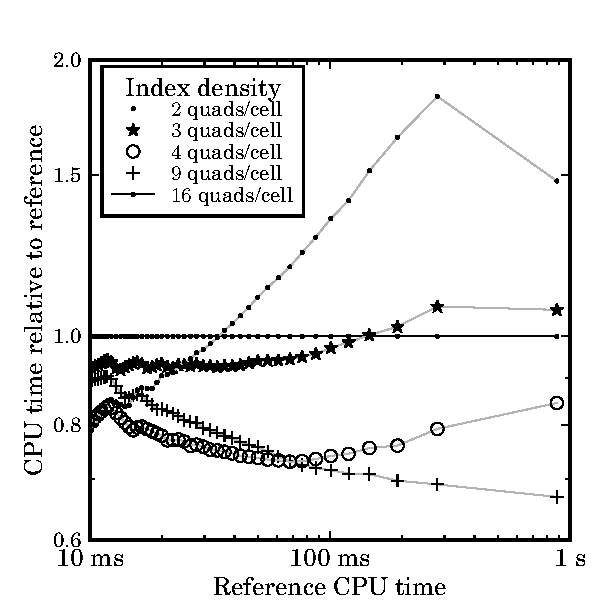
\includegraphics[width=1.000000\figunit]{sdss-density-reltime}}
\newcommand{\sdssdensitytimefig}{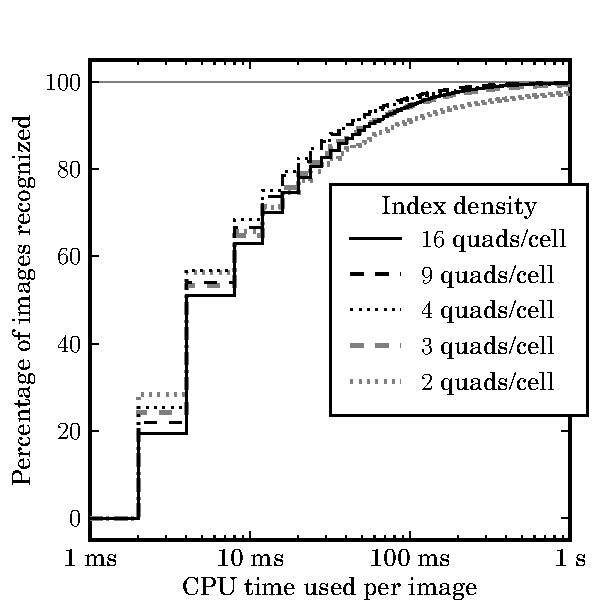
\includegraphics[width=1.000000\figunit]{sdss-density-time}}
\newcommand{\sdsstriquinttable}{\newlength{\cw}
\settowidth{\cw}{\textbf{Percentage of images recognized}}
\begin{tabular}{|c|D{.}{.}{3.2}|D{.}{.}{3.2}|D{.}{.}{3.2}|}
\hline
\multicolumn{1}{|c|}{\textbf{CPU time}} &\multicolumn{3}{c|}{\textbf{Percentage of images recognized}} \\
\cline{2-4}
\multicolumn{1}{|c|}{(per image)} & \multicolumn{1}{c|}{\makebox[0.35\cw][c]{Triangles}} & \multicolumn{1}{c|}{\makebox[0.35\cw][c]{Quads}} & \multicolumn{1}{c|}{\makebox[0.35\cw][c]{Quints}} \\
\hline
\makebox[\pointonesec][r]{$0.1$ s} & 0.20  & 57.45  & 23.35 \\
\makebox[\pointonesec][r]{$1$ s} & 28.07  & 92.20  & 36.67 \\
\makebox[\pointonesec][r]{$10$ s} & 78.58  & 99.28  & 72.75 \\
\makebox[\pointonesec][r]{$100$ s} & 99.15  & 99.33  & 95.08 \\
\makebox[\pointonesec][r]{$1000$ s} & 99.97  & 99.33  & 96.25 \\
\hline
\end{tabular}
}
\newcommand{\sdsstriquintntrynmatchfig}{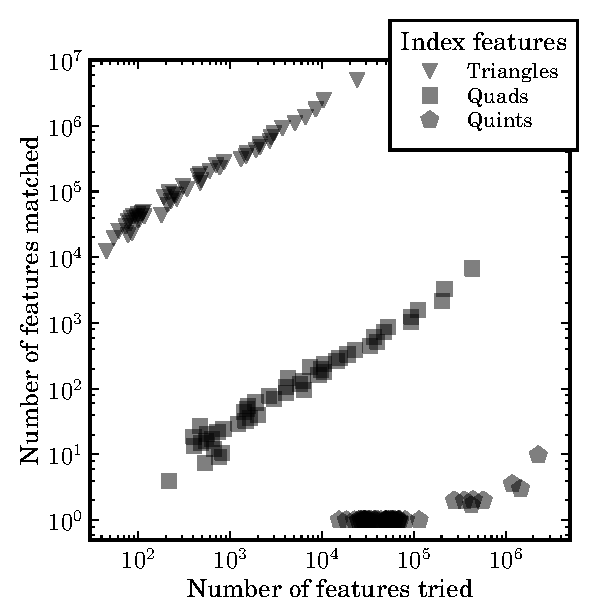
\includegraphics[width=1.000000\figunit]{sdss-triquint-ntrynmatch}}
\newcommand{\sdsstriquinttimefig}{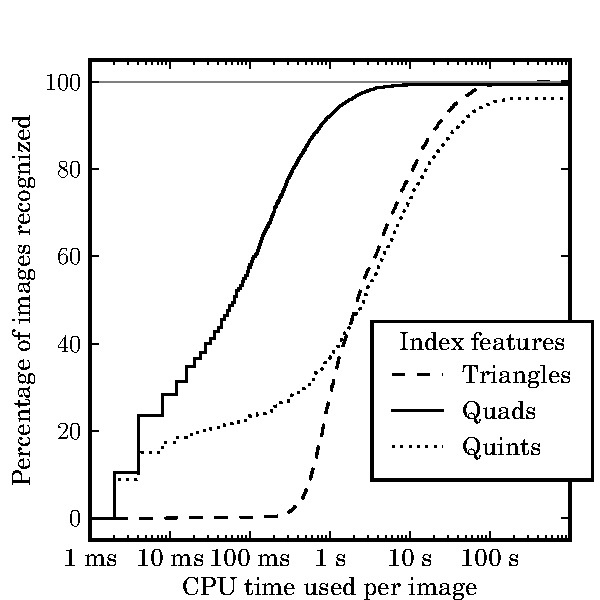
\includegraphics[width=1.000000\figunit]{sdss-triquint-time}}
\newcommand{\galextable}{\begin{tabular}{|c|D{.}{.}{3.2}|}
\hline
\multicolumn{1}{|c|}{\textbf{CPU time (per image)}} &\multicolumn{1}{c|}{\textbf{Percentage of images recognized}} \\
\hline
\makebox[\pointonesec][r]{$1$ s} & 74.46 \\
\makebox[\pointonesec][r]{$10$ s} & 93.56 \\
\makebox[\pointonesec][r]{$100$ s} & 98.95 \\
\makebox[\pointonesec][r]{$1000$ s} & 99.74 \\
\hline
\end{tabular}
}
\newcommand{\galexcputimefig}{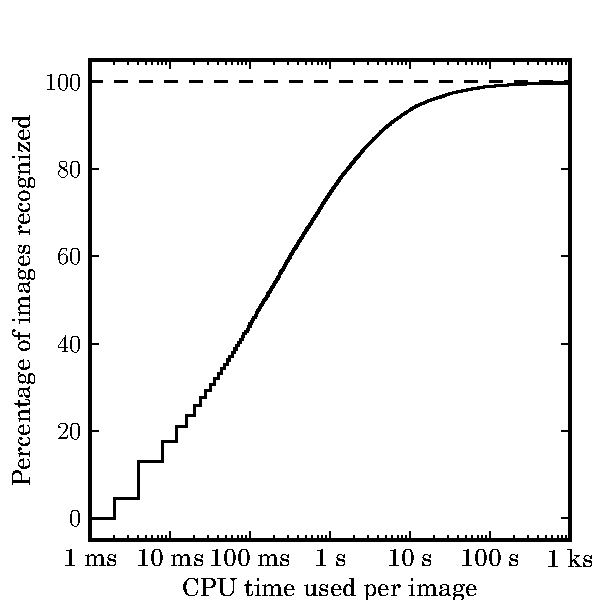
\includegraphics[width=1.000000\figunit]{galex-cputime}}
\newcommand{\galexindexidfig}{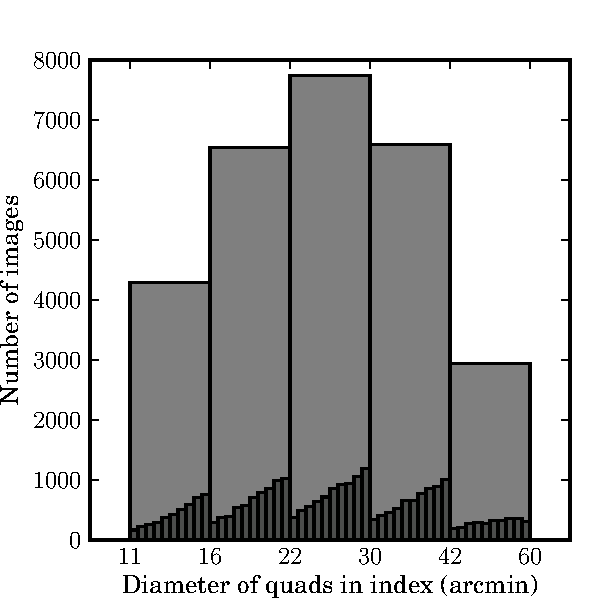
\includegraphics[width=1.000000\figunit]{galex-indexid}}
\newcommand{\galexquadfig}{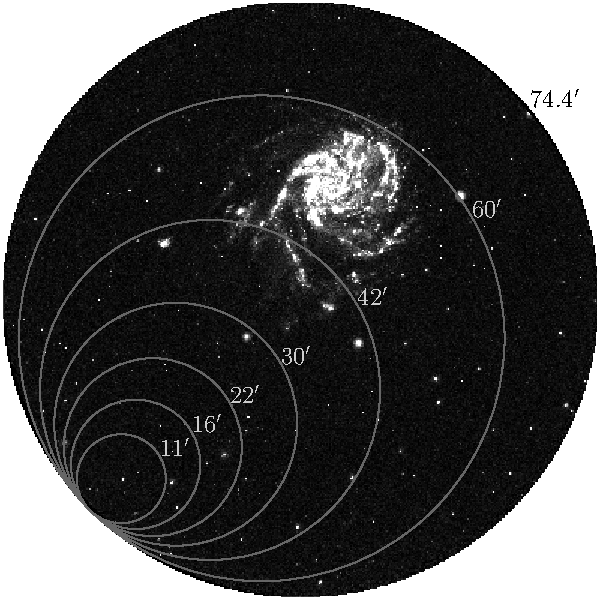
\includegraphics[width=1.000000\figunit]{galex-quad}}
\newcommand{\sdssquadfig}{\includegraphics[width=1.000000\figunit]{sdss-quad}}
\newcommand{\aegisacsquadfig}{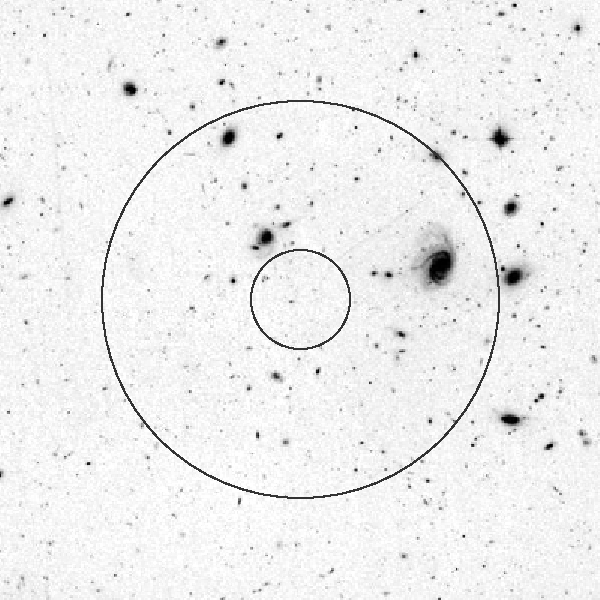
\includegraphics[width=1.000000\figunit]{aegis-acs-quad}}
\newcommand{\aegisacsquadsizesfig}{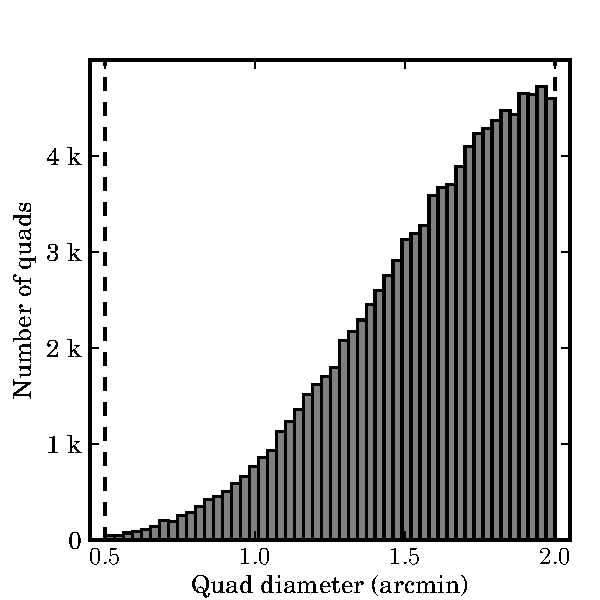
\includegraphics[width=1.000000\figunit]{aegis-acs-quadsizes}}
